\chapter{Introduzione a Moon Cloud}
\label{chp:01-introduction}
In questo capitolo verrà descritto in modo più approfondito il funzionamento della piattaforma Moon Cloud e unitamente al 
motivo dell'implementazione della soluzione proposta.

\section{Moon Cloud overview}
La diffusione di sistemi \textit{Information and Communications Technology} (acronimo ICT) ha avuto luogo nella maggiorparte degli ambienti 
lavorativi e privati in termini di servizi offerti, automazione di processi e incremento delle performance. L'uso di questa tecnologia 
ha assunto importanza a partire dagli anni novanta come effetto del boom di Internet e al giorno d'oggi le professionalità legate al
mondo dell'ICT crescono in numero e si evolvono per specificità, per operare in ambienti fortemente eterogenei ma sempre più 
interconnessi fra di loro come il Cloud Computing, i Social Newtwork, il Marketing Digitale, i Sistemi IoT, la Realtà Virtuale, etc.

Il Cloud Computing ha portato un rivoluzionario paradigma nella creazione di un nuovo business virtuale accessibile in qualunque momento
e in qualunque luogo; esso sfrutta le tecnologie messe a disposizione dai sistemi ICT come le operazioni di virtualized computing,
internet e distributed computing, provvedendo un sistema integrato molto potente. Google, Microsoft, Amazon sono un esempio di 
aziende che forniscono servizi di Cloud Computing in business ICT. Si può definire il Cloud Computing come l'abilità di accedere a 
risorse (come database o applicazioni) in tutto il mondo attraverso una rete in poco tempo.

Gli immensi benefici del Cloud in termini di flessibilità, consumo delle risorse e gestione semplificata, la rende la prima scelta per 
utenti e industrie per il deploy dei loro sistemi IT. Tuttavia il Cloud Computing solleva diverse problematiche legate alla mancanza di 
fiducia e trasparenza dove i clienti necessitano di avere delle garanzie sui servizi Cloud ai quali si affidano; spesso i fornitori di 
questi servizi non fornisco ai clienti le specifiche riguardanti le misure di sicurezza messe in atto.

Negli ultimi anni, sono state sviluppate tecniche e modi per rendere sicuri questi sistemi e proteggere i dati degli utenti, portando 
alla diffusione di approcci eterogenei che incrementaro la confusione negli utenti.
Tecniche tradizionali di verifica della sicurezza basati su metodi di analisi statistica non sono più sufficenti e devono essere integrati 
con processi di raccolta di prove (in inglese evidence) da sistemi Cloud in produzione e funzionanti. 
In generale il \textit{Cloud Security} definisce i modi, come criptazione e controllo degli accessi, per proteggere attivamente gli asset 
da minaccie interne ed esterne, e fornire un ambiente in cui i clienti possano affidarsi e interagire in totale sicurezza. 
Tutto questo non basta a rendere il Cloud degno di fiducia e trasparente, per questo sono state introdotte tecniche di
\textit{Security Assurance}, delle garanzie che permettono di ottenere la fiducia necessaria nelle infrastrutture e/o nelle 
applicazioni di dimostrare il rispetto di certe proprietà di sicurezza, e che operino normalmente anche se subiscono attacchi; grazie 
alla raccolta e allo studio di evidence è possibile che venga accertata la validità e l'efficenza delle proprietà di sicurezza messe in 
atto.

Il prezzo che si paga per i benefici di questa tecnologia è dato dall'incremento di violazioni di sicurezza, che oggigiorno 
preoccupa tutte le aziende e di conseguenza anche i loro clienti, con l'incremento del rischio di fallimento per i servizi più importanti 
dovuti a violazioni della privacy e al furto di dati. 
\\
Il mercato sta lentamente notando che non è l'inadequamento tecnologico dei sistemi di sicurezza che incrementa il rischio delle 
violazioni di sicurezza; piuttosto, la mal configurazione e l'errata integrazione di questi sistemi nei processi di business. 
\cite{cloud-Platform-for-ICT-Security-Governance}
L'utilizzo di sistemi di sicurezza e di controllo migliori non garantisce in modo assoluto la sicurezza dell'infrastruttura; 
per garantire ciò è necessario implementare un processo continuo di diagnostica e verifica della corretta configurazione dei controlli, 
supervisionando il loro comportamento, accertandosi che sia quello aspettato.

Il \textit{Security Assessment} diventa allora un aspetto importante specialmente negli ambienti Cloud e IoT. Questo proccesso, costituito
da un insieme di attività mirate alla valutazione del rischio in sistemi IT, deve essere portato avanti in modo continuo e olistico, per 
correlare le evidence raccolte da sempre maggiori meccanismi di protezione. \cite{mooncloud-semi-automatic-and-trustworthy}
\\
Moon Cloud è una soluzione PaaS (acronimo inglese di Platform as a Service) che fornice una piattaforma B2B (Business To Business) 
innovativa per verifiche, diagnostiche e monitoraggio dell'adeguatezza dei sistemi ICT rispetto alle politiche di sicurezza, in modo 
continuo e su larga scala. Moon Cloud supporta una semplice ed efficente \textit{ICT Security Governance}, dove le politiche di sicurezza 
possono essere definite dalle compagnie stesse (a partire da un semplice controllo sulle vulnerabilità a linee guida di
sicurezza interna), da entità esterne, imposte da standard oppure da regolamentazioni nazionali o internazionali.
\\
La sicurezza di un sistema o di un insieme di asset dipende solo parzialmente dalla forza dei singoli meccanismi di protezione isolati
l'uno dall'altro; infatti, dipende anche dall'abilità di questi meccanismi di lavorare continuamente in sinergia per provvedere una 
protezione olistica.
In più, quando i sistemi Cloud e i servizi IoT sono coinvolti, le dinamiche di questi servizi e la loro rapida evoluzione rende il 
controllo dei processi all'interno dell'azienda e le politiche di sicurezza più complesse e prone ad errori.
\\
I requisiti ad alto livello fondamentali per poter garantire le Security Assurance sono:
\begin{description}
	\item[sistema olistico] è richiesta una visione globale e pulita dello status dei sistemi di sicurezza; inoltre è cruciale 
	distribuire lo sforzo degli specialisti in sicurezza per migliorare il processo e le politiche messe in atto. Si parte da 
	delle valutazioni fatte manualmente a quella semi-automatiche che vengono usate per ispezionare i meccanismi di sicurezza. 
	\item[monitoraggio continuo ed efficiente] è necessario un controllo continuo che valuti l'efficenza dei sistemi di sicurezza 
	per ridurre l'impatto dell'errore umano, soprattutto dal punto di vista organizzativo. La coesistenza di componenenti in conflitto o
	la mancata configurazione dovuta al	cambiamento dell'ambiente possono essere scenari che richiedono un monitoraggio e un 
	aggiornamento continuo.
	\item[singolo punto di management] avere un solo punto d'accesso in cui poter gestire tutti gli aspetti relativi alla sicurezza, 
	permette di avere sotto controllo le politiche di sicurezza. Inoltre disporre di un inventario degli asset da proteggere permette di
	poter conoscere quali meccanismi di protezioni applicare.
	\item[reazioni rapide a incidenti di sicurezza] spesso la reazione ad incidenti di sicurezza è ritardata da due fattori: il tempo 
	richiesto per rilevare l'incidente e il tempo per analizzare il motivo dell'accaduto; e avere un sistema che implementa un monitoraggio
	continuo permette di venire a conoscenza di questi problemi in breve tempo e agire di conseguenza.
	\label{list:security-assurance-fondamentals}
\end{description}


Moon Cloud è basato su una tecnica di Security Assurance garantendo che tutte le attività aziendali si compiano seguendo i requisiti 
prestabiliti da appropriate politiche e procedure precedentemente definite.

Viene definita una \textit{Security Compliance Evaluation}, un processo di verifica a cui un target viene sottoposto e il cui risultato 
deve soddisfare i requisiti richiesti da standard e politiche. A partire da questi processi di controllo, che devono a loro volta essere 
affidabili, si ottendo delle evidence; queste ultime possono essere raccolte monitorando l'attività del target oppure, come già 
menzionato, sottoponendo il target a scenari critici o di testing.
In particolare, una Security Compliance Evaluation è un processo di verifica dell'uniformità di un certo target a una o più politiche 
attraverso una serie di controlli che a seconda del valore booleano (successo pari a 1 o insuccesso pari a 0) associato ad ogni controllo viene prodotto 
un valore booleano per le politiche; se un target supera tutti i controlli, quindi tutti i valori booleani associati ad ogni controllo
è pari al successo, a cui è sottoposto allora significa che rispetta la politica scelta. 

\begin{figure}
	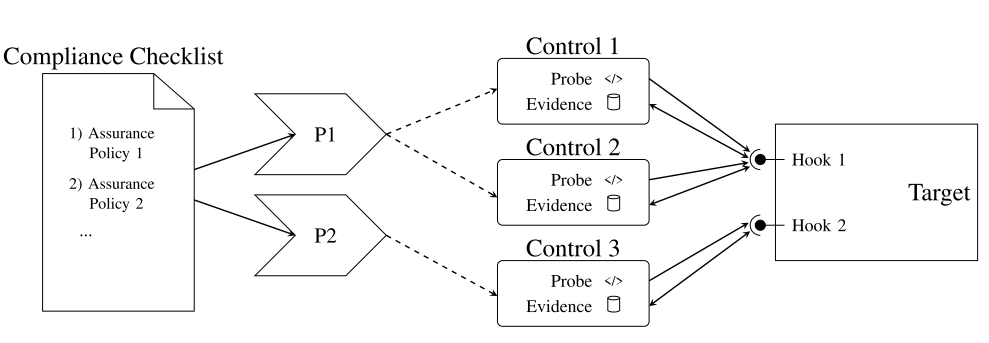
\includegraphics[scale=0.5]{images/Security_Compliance_Evaluation.png}
	\caption{Security Compliance Evaluation}
	\label{fig:Security_Compliance_Evaluation}
\end{figure}

\newpage

\section{Processo di Evaluation}
Moon Cloud implementa il processo di Security Compliance Evaluation in Figura \ref{fig:Security_Compliance_Evaluation} usando controlli 
di monitoraggio o di test personalizzabili. Inoltre garantisce, oltre a tutti i requisisti ad alto livello elencati precedentemente 
\ref{list:security-assurance-fondamentals}, anche i seguenti:
\begin{description}
	\item Moon Cloud è una piattaforma Cloud centralizzata presentando una visione olistica dello stato di sicurezza di un dato sistema.
	\item Moon Cloud implementa un sistema di Security Assurance Evidence-based continuo, implementato come processo di Compliance,
	basato su politiche custom o standard.
	\item Moon Cloud è offerto come un servizio (PaaS), dove le attività di Evaluation possono essere facilmente ed efficentemente 
	configurate su un target asset, senza l'intervento dell'uomo.
	\item Moon Cloud permette di schedulare delle ispezioni automatiche, grazie all'inventario di asset protetto.
	\item Moon Cloud Evaluation Engine può ispezionare dall'interno un sistema, gestendo così delle minaccie interne; permettendo anche 
	reazioni rapide a incidenti di sicurezza e veloci rimedi, grazie alla raccolta continua di evidence. 
\end{description}


In generale, l'architettura di Moon Cloud è costituita da un'Assurance Manager che gestisce i processi di Evaluation attraverso un set di 
\textit{Execution Cluster}; ognuno dei quali gestisce ed esegue un set di probe che collezionano le evidence necessarie per effettuare 
i processi di valutazione.
Tutte le attività di collezione sono eseguite dal probe, ognuno dei quali è uno script Python fornito come una singola immagine di Docker, 
che viene inizializzata quando viene triggerata una Evaluation ed è distrutta quando il processo di Evaluation è terminato.
\\
Accedendo alla piattaforma di Moon Cloud, l'utente può definire le proprie politiche di sicurezza e attività di Evaluation come 
espressioni booleane di controlli di sicurezza e altre politiche predefinite. Una volta che una politica viene definita, l'utente può 
decidere quando schedulare l'Evaluation; e nel momento in cui un processo di Evaluation viene inizializzato, tutti i controlli vengono 
eseguiti e i risultati dell'espressioni booleane vengono memorizzati e restituiti all'utente. A questo punto l'utente può accedere a 
questi risultati a diversi gradi di precisione: una visione sommaria e generale di tutte le politche implentate e dello stato generale 
del sistema di sicurezza, al risultato di una specifica politica oppure alle evidence raccolte per una Evaluation.

Per poter rendere ancora più intuituivo e semplice da utilizzare un sistema di questa importanza, si è pensato di introdurre un sistema
che possa raccomandare agli utenti, in base agli asset che vuole proteggere e monitorare, una serie di Evaluation o politihe da
applicare in quei casi; questo permette anche a utenti meno esperti di poter configurare in modo rapido ed efficente dei meccanismi di
protezione da minaccie.